%!TEX root = ../thesis.tex
%*******************************************************************************
%*********************************** First Chapter *****************************
%*******************************************************************************

\chapter{Introduction \label{chap:1}}  %Title of the First Chapter

\ifpdf
    \graphicspath{{Chapter1/Figs/Raster/}{Chapter1/Figs/PDF/}{Chapter1/Figs/}{Chapter1/Figs/Vector/}}
\else
    \graphicspath{{Chapter1/Figs/Vector/}{Chapter1/Figs/}}
\fi


A new field of research related to both material science and condensed matter physics has been formed since the synthesis of graphene in 2004 \cite{Novoselov666,Novoselov26072005}. Graphene is a sheet of carbon atoms in a crystal form having a single atom thickness. Given the thin plane-like structural nature of this type of materials the field is named two-dimensional (2D) material. The synthesis itself together with the phenomenal properties of graphene has leaded to a Nobel Price in physics rewarded to Andre Geim and Konstantin Novoselov in 2010 \cite{Geim2007}. Since then, the field is expanding with the involvement of researchers not only from young community, but also from experts who have been working on graphene-related materials like graphite, fullerenes and carbon nanotubes. As a result, researches focused on graphene and related topics increasing with unprecedented speed, see \autoref{fig:grpapers}. While a part of these effects has been making to explore more on the graphene itself and its applications, the other parts were put on discovering new 2D materials like graphene. It has been evidenced from graphene, same material having different dimensionality can have different properties. Therefore, many materials with hidden properties which will only manifest themselves at other dimensions yet to be discovered. 


\begin{figure}[htbp!] 
\centering  
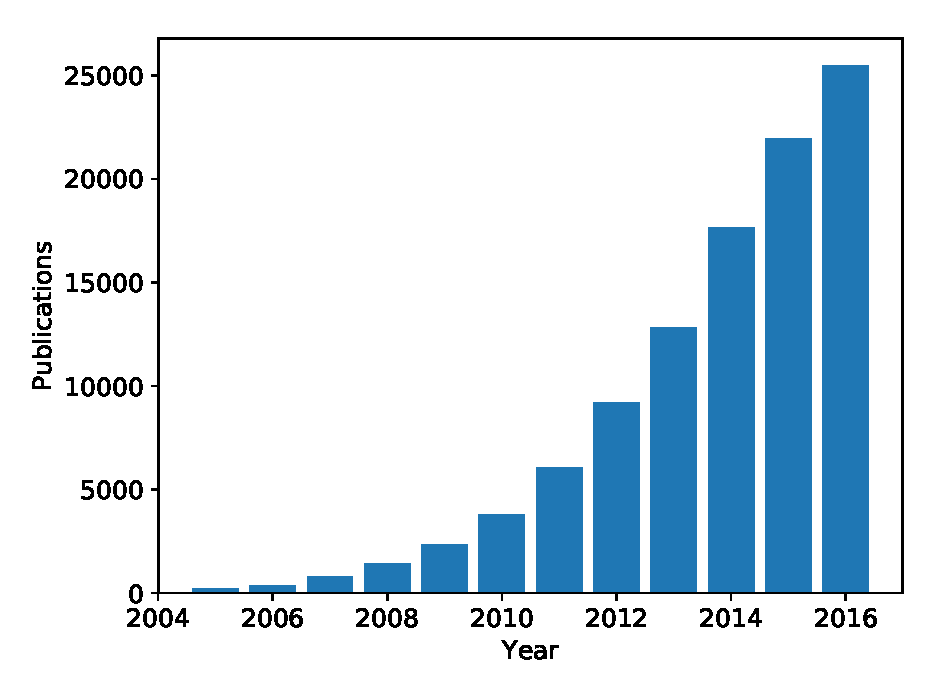
\includegraphics[width=0.8\textwidth]{graphene_papers.eps}
\caption[Graphene publications]{Graphene related publications and patents during the last decade. Data source: ISI Web of Science and PATENTSCOPE. \protect\footnotemark }  
\label{fig:grpapers}
\end{figure} 

On the other hand, with the advent of powerful supercomputer facilities, calculations that seems impossible to finish in a reasonable time now has been made possible. The accuracy of such calculations is the most crucial aspect of computational physics, especially when the results are utilized to predict the real materials properties. To make the time spend on costly supercomputer valuable, researchers and programmers have been making important progress to make sure theories and its implementation are correct and the results they yield are within acceptable precision. Equipped with these tools, theoretical predictions have served well on discovering unexplored properties and applications of the materials. Moreover, detailed characterizations at atomic scale benefits the experimental results as well, or even to explain the unexpected outcomes.

Considering all mentioned, it is a sound approach to apply the state-of-the-art computational methods that accompanied with high-performance supercomputer facilities to investigate the physical properties of novel 2D materials. This thesis were initiated to this end and it is a summary of several works which has been accomplished during my PhD study. The thesis is organized as followed: For the rest of this chapter, I will first introduce graphene and some post-graphene materials that discovered right after graphene and, briefly, several well-known methods used to synthesis 2D materials. The following \autoref{chap:2} will present the computational methods, the theory and the implementations of them in available software packages. In \autoref{chap:3}, I will discuss several general properties of 2D materials. The next two chapters will be the main results from my works. Starting from specific properties targeting at specific novel 2D materials in \autoref{chap:4}, and followed by modification of physical properties of 2D materials in \autoref{chap:5}. Overlaps of materials themselves and their properties are inevitable between sections yet it will be minimized, such that each section will have a unique topic. 

\footnotetext{Publication and patent results are obtained by searching for "graphene" in the topic field of Web of Science and the title field of PATENTSCOPE, respectively.}

\section{Graphene}

Graphene is composed of carbon (C) atoms arranged on a honeycomb lattice in a single atomic layer. Graphene is one of layers that construct graphite, see \autoref{fig:gra_grap}. These layers in graphite are stacked on top of another through weak physical bonding, whereas within each layer C atoms are hold together by strong chemical bonding. As a result, it is possible to just isolate single layer from graphite without damaging the layer itself. 

\begin{figure}[htbp!] 
\centering  
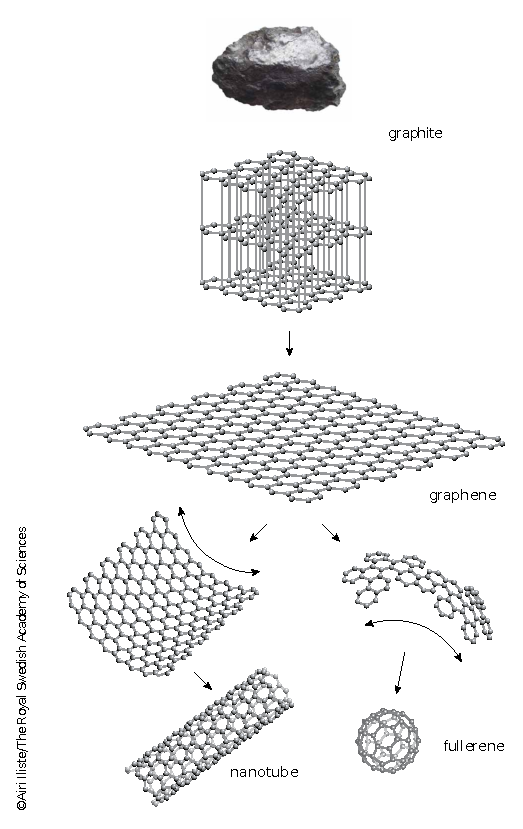
\includegraphics[width=0.7\textwidth]{gra_grap.eps}
\caption{Relation of graphite, graphene, fullerene and nanotube. Image source: the Nobel prize in physics 2010 \cite{gra_grap}. }  
\label{fig:gra_grap}
\end{figure} 


\subsection{History}

The story of graphene can be traced back to the discover of graphite around 1564 in England\cite{petroski1990pencil}. Ever since, people have been using the graphite, the tip of a pencil, for writing and drawing. The black trace left behind by pencil they are actually stacks of graphite and graphene, by chance even a single layer graphene can present.  Apart from being a part of a pencil, graphite certainly has been holding a more important position in technology and industry due to its rich chemistry, low friction, high electrical and thermal conductivity etc. . On the other hand, the synthesis of single layer graphene seems to be discouraged by both experimental and theoretical limitation. On the experiments, there have been attempts\cite{Krishnan1997,Ohashi1997,Dresselhaus2002,Shioyama2001} to isolate graphene from graphite or even grow it on a substrate. However, they were mostly failed on the control of the number of layers and identifying graphene itself.  Addition to these experimental difficulties, on the theory, it was believed that strictly 2D material should not exist due to a divergence in the thermal fluctuation in 2D materials that will make them not stable \cite{Peierls1935,Landau1937,Mermin1968}. Nevertheless, graphene was still considered as a theoretical model. for example, \citet{Wallace1947} was the first one to study the band structure of graphene \cite{CastroNeto2009} and found some of the interesting properties like semimetallic band structure. 

Although not in the form of graphene, the single atomic layer of graphite has been already seen and studied in other forms, e.g. fullerenes and nanotubes, see \autoref{fig:gra_grap}. These material usually contain certain types of characteristic defects that differ it from graphite.  Fullerene is a C molecule has a quasi-spherical hollow ball shape. It is composed of both six- and five-folded C rings, where the latter give positive curvature and made closed surface possible. The resulting shape resembles a football\cite{Kroto1985,Lamb1990}. The Nobel prize in chemistry of year 1996 was award to Harold W. Kroto, Robert F. Curl and Richard E. Smalley for their discovery of fullerene. Another important type of carbon allotrope, carbon nanotubes\cite{Iijima1993}, was discovered using arc-discharge method\cite{Lamb1990} which was originally designed to produce a large quantity of fullerenes. Despite sharing similar production method, carbon nanotubes are actually more close to graphene than fullerene due to the absence of pentagonal C rings in the former two. A carbon nanotube can be construct by rolling up graphene sheet into a hollow tube as its name suggested. Carbon nanotubes are observed to have micrometer in lengths and nanometre in diameters and having either metallic or semiconducting nature depending on its edges. They possess superior mechanical properties. Individual nanotube has a Young's modulus of 0.64 TPa and it is 56 times stronger than steel wire\cite{Baughman787}.

In 2004, the situation has changed completely for graphene with the successfully isolated single layer graphene from graphite by A. K. Geim and K. S. Novoselov at Manchester University using a simple micromechanical cleavage method. The key ingredient for success in this case as compared to the previous failures\cite{Krishnan1997,Ohashi1997}, except for the sophisticated experimental control, is that the Si wafer under the graphene made it easier to identify graphene\cite{Geim2007}. The synthesis of graphene itself already is a ground-breaking achievement, however, what excited the researcher the most is the extraordinary properties of graphene. In the following section, I will summarized some of them to illustrate this point.

\subsection{Physical properties}

As mentioned previously, graphene is the single atomic layer of graphite. It posses an interesting structure with high symmetry which many of its properties are attributed to. Each C atom has three neighbours to make chemical bonds. Because of this, C atoms are arranged in a honeycomb lattice\footnote{honeycomb lattice is not a Bravais lattice.}, or a hexagonal Bravais lattice with two atoms per site, see (a) in \autoref{fig:gra_band}. Graphene has uniform bond lengths of 1.42\AA~ and uniform bond angles of 120\textdegree. The band structure which characterizes the electronic properties of graphene has been calculated by P. R. Wallace in 1947 \cite{Wallace1947}. He discovered that graphene is a semimetal with conduction band minimum (CBM) and valence band maximum (VBM) only touch each other at the K and K' points in the first Brillouin zone as shown in (b) and (c) in \autoref{fig:gra_band}. The energy-momentum dispersion is approximately linear in the vicinity of K and K' points. Due to this, the electron and hole in those states behave differently as they do in quadratic band. Several consequences of this can be concluded. First of all, considering the linear energy momentum relation, particles can be regard as Dirac particles and they are governed by relativistic Dirac equation\cite{Novoselov2005}, and they travel at constant speed of \si{10^6m/s}. Hence, the K and K' points are referred as Dirac points, their vicinities are called Dirac cones. Secondly, the carrier concentration can be tuned continuously from electron to hole with a perpendicular electric field\cite{Geim2007}. Thirdly, the carrier in graphene can tunnel through finite height potential it normally incident to without reflection — Klein tunnelling\cite{Katsnelson2006}. Fourthly, under magnetic field, zero energy Landau level appears, and the large energy interval between zero to first level made it possible to observe quantum Hall effect at room temperature \cite{Novoselov1379}, etc..

\begin{figure}[htbp!] 
\centering  
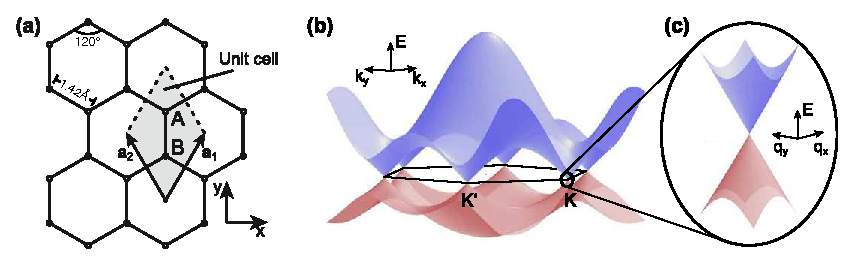
\includegraphics[width=\textwidth]{gra_lat_band.eps}
\caption[Graphene lattice and band structure.]{(a) Graphene honeycomb lattice composed of A and B hexagonal Bravais sublattices. (b) Band structure of graphene where CBM and VBM touch each other only at the K and K' points. (c) Approximately linear dispersion around the K and K' points. Image source: \cite{Guttinger2012}. }  
\label{fig:gra_band}
\end{figure} 

Graphene delivers more than just an interesting electronic property. For example, evidencing the extraordinary mechanical properties, graphene has a Young modulus E = 1Tpa and intrinsic strength of 130 Gpa\cite{Lee385}. This makes graphene the strongest material ever measured. More than 300 times stronger than steel and four times harder than diamond. Carrier high mobility is another exciting feature that has more applicative importance in electronic devices. Free standing graphene without subtract attached has been reported to has mobility of 230,000 \si{cm^2/Vs} at low temperature\cite{Bolotin2008a} and 120,000 \si{cm^2/Vs} at 240 Kelvin, the latter value is higher than any known semiconductor\cite{Bolotin2008b}. In addition, the thermal conductivity of graphene can reach up to 5000 \si{W/mK} at room temperature, which is 20 times higher than copper\cite{balandin2008}. However, having a zero band gap means the application of graphene in digital logic gates is limited. The current controlled by the gate bias can not be turned off completely which would otherwise deliver distinct signal from when it is on. Efforts on band gap opening have been made, from substrate induction\cite{Ci2010,zhou2007}, bilayer graphene\cite{mccann2006,castro2007}, chemical adsorption\cite{Elias2009,Jeon2011}, and chemical doping\cite{zhou2008} to quantum confinements\cite{Nakada1996,Barone2006}.  While doping and adsorption usually come with a cost of reducing mobility by introducing scattering centres, chemically pure bilayer graphene and nanoribbon are thought to be promising approaches to open band gap as well as, to a great extend, preserve graphene's superior intrinsic properties.

\section{Post-graphene materials and their general properties}

Excitements in the exploration of graphene properties drive the force to discover more types of 2D materials. Researchers have taken different approaches to this end. On one hand, aiming to open a band gap in graphene, chemical functionalizations on graphene have been carried out with adsorption of hydrogen, fluorine and oxygen, and they results in graphane, fluorographene and graphene oxide, respectively; On the other hand, inspired by graphite's layer structure, layered materials are brought to the attention to isolate its single layer just as it has done for graphene. In this section, I will introduce some of these early post-graphene materials and their physical properties in general.

\subsection{Functionalized graphene}

\subsubsection{Graphane}

The fully hydrogenation of graphene gives a 2-D hydrocarbon called graphane. It can synthesized either by reduction of graphite then hydrogenation of left product (graphene, carbon nanotubes or graphite oxide) with liquid-based\cite{Yang2012} or gas-based\cite{Burgess2011} environments, or growing by chemical vapour deposition\cite{wang2010}. 

graphane is not flat as graphene. In fact, the bonding character changed from sp$^2$ hybridization to sp$^3$, which gives buckled structure, see \autoref{fig:gra_h}. Neighbouring H atoms locate at the different sides of graphane plane. Among different phases of graphane, chair structure is the ground state. Others phases are metastable state like: boat, twist-boat and twist-boat-chair\cite{Samarakoon2009}. The C-C bond length in the chair structure is 1.52 \AA~lager than that in graphene. graphane is a semiconductor with 3.5 eV band gap in the chair form. Band gap is reported scales almost linearly with the hydrogen coverage\cite{Ilyin2011}. The 2D Young's modulus of graphane is estimated 245 \si{N/m}\cite{Munoz2010}, smaller than 340 \si{N/m} in graphene. The incomplete coverage of H atoms on graphene gives hydrogenated graphene. It has ferromagnetic magnetic state\cite{Zhou2009}, tunable band gap\cite{Shkrebtii2011} and reversible hydrogenation\cite{Elias2009}. 

\begin{figure}[htbp!] 
\centering  
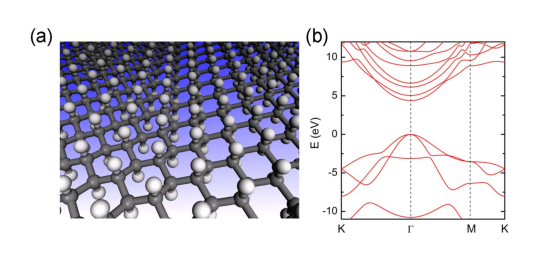
\includegraphics[width=1\textwidth]{graphane.eps}
\caption[Atomic and electronic structure of graphane]{(a)The chair structure of graphane. The white balls are the H atoms and the grey ones are the C atoms. Image source: \cite{Sofo2007}. (b) Band structure of chair graphane. Image source: \cite{leenaerts2010}}  
\label{fig:gra_h}
\end{figure} 

\subsubsection{Fluorographene}

More stronger binding between external atom and C atom can be realized using fluorine atom for adsorption . A full fluorinated graphene is called fluorographene, and it can be regards as a single layer of graphite fluoride. Actually, sonochemical exfoliation of fluorographene from graphite fluoride is one of the ways to synthesis it, see \autoref{fig:gra_f}\cite{Zhu2013}. Fluorographene has a similar structure as graphane due to same sp$^3$ hybridization, and it also has different isomers where the again the chair type is the ground state configuration\cite{samarakoon2011}. The unit cell of fluorographene is around 1\% larger than that of graphene\cite{nair2010}. The formation energy of fluorographene is around 0.5 eV per fluorine atom lower than that of graphane per hydrogen atom\cite{Jeon2011}. The band gap of fluorographene is larger than 3 eV from optical measurement\cite{nair2010,Jeon2011}, and band structure is similar to that of graphane with a band gap at the $\Gamma$ k-points. The 2D Young's modulus of Fluorographene is 100 \si{N/m} and the intrinsic strength is about 15 \si{N/m}. They both more than two times less than those for graphene due to weaker sp$3$ bonds in fluorographene\cite{nair2010}.

\begin{figure}[htbp!] 
\centering  
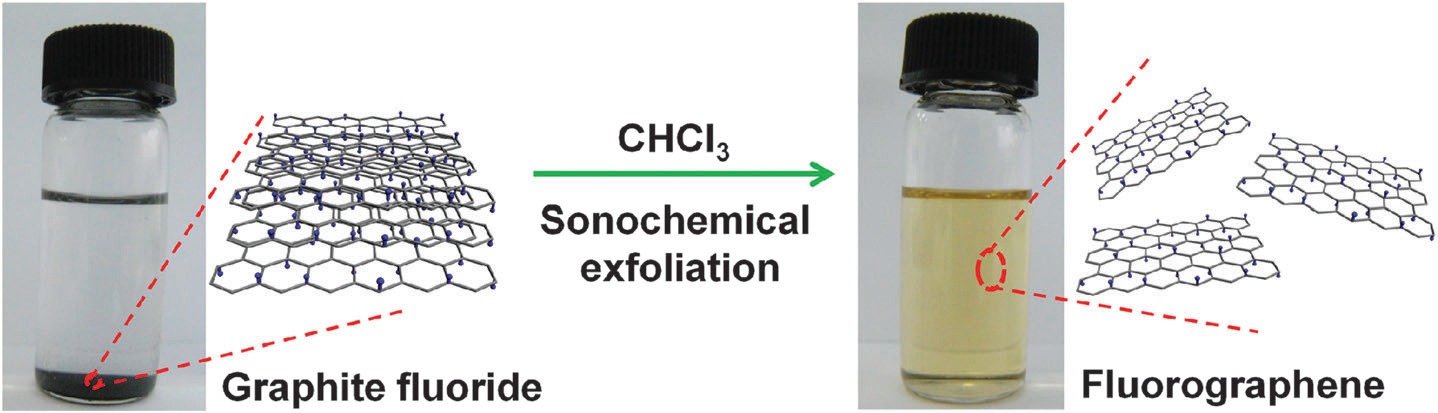
\includegraphics[width=1\textwidth]{fluorographene.png}
\caption{Graphite fluoride to fluorographene. Image source:\cite{Zhu2013}}  
\label{fig:gra_f}
\end{figure} 

\subsection{Group IV 2D materials}

In analogues to graphene, 2D material made of only single element from other members of group IV have been also proposed and synthesized. They are silicene, germanene, stanene made of silicon (Si), germanium (Ge) and tin (Sn) atoms, respectively. They generally suffer from less stability with respect to graphene. The free standing form of these material are hard to make, instead they usually need ordered substrates to support them. Therefore, the measurements done on these type of system can not exclusively speak for the target material, the influence of the substrate is not negligible\cite{Lin2013}. This will in turns hinder the accurate characterization of the properties. Despite these experimental difficulties, theoretical studies have more freedom to investigate their physical properties. One of the most important differences of these materials as compared to graphene is their not-flat buckled structure, see \autoref{fig:silicene}. The buckling parameters $\delta$ is defined as the interlayer distance of layers at different 2D atomic planes. According to calculations, $\delta$ is 0.45\AA~for silicene, 0.69\AA~for germanene and 0.85 \AA~for stanene\cite{matthes2013}. This change corresponds to a more sp$^3$ character in the orbitals, and it increases with the atomic radius. 

\begin{figure}[htbp!] 
\centering  
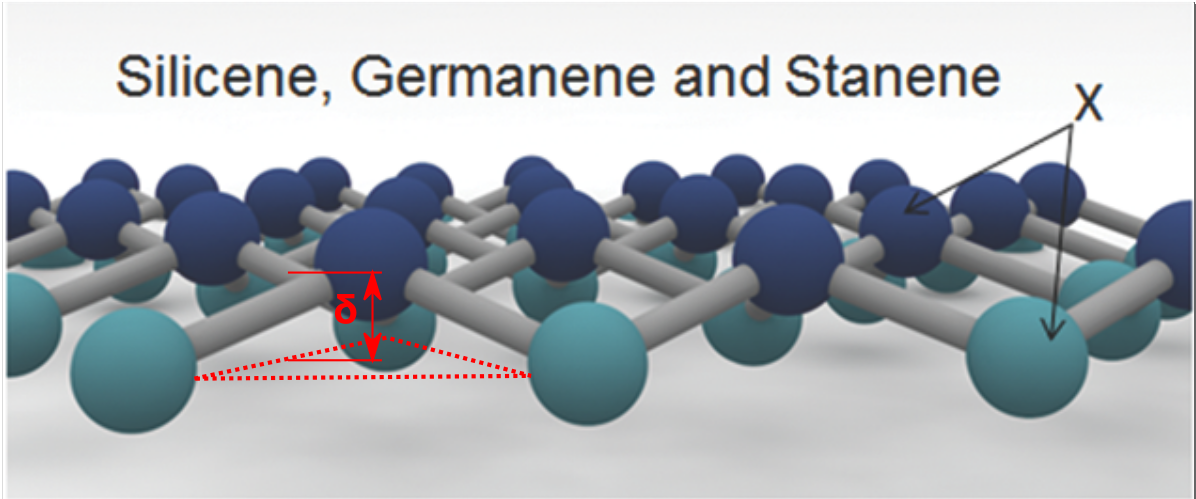
\includegraphics[width=0.9\textwidth]{silicene_structure.png}
\caption{Buckled hexagonal crystal structures of 2D group IV materials (X = Si, Ge, and Sn). Different colors represent different 2D planes and their distance is the buckling parameter $\delta$. Image adapted from:\cite{Balendhran2015}}  
\label{fig:silicene}
\end{figure} 


Although having a buckled structure, these materials also posses Dirac points with linear energy momentum dispersion around it\cite{Garcia2011}.  However, as stated before, the substrate where the materials are supported will induce symmetry broken which leads to the lost of Dirac character for particles\cite{Lin2013}. Moreover, spin-orbit coupling (SOC) in these materials are predicted to be larger than that in graphene due to larger atomic weights. With inclusion of SOC, this corresponds to 1.9 meV band gap in silicene  and 101 meV of that in stanene\cite{matthes2013}. The mechanical stiffness and strength are low as compared to graphene and has a reducing trend with increasing atomic number in this group. This is partially due to the less energetically costly bond angle deformation in the buckled structure upon load rather than bond stretching in a flat structure\cite{Manjanath2014}. For example, silicene has a 2D Young's modulus around 62 \si{N/m}, that is four times smaller than graphene. Another important difference of these materials from graphene regards the realization of monolayer. The lack of layered bulk materials for the former ones made the mechanical exfoliation inapplicable for them, which is believed to produce the highest quality sample otherwise. Therefore, methods used in this case are either bottom-up decomposition techniques onto highly ordered substrates\cite{vogt2012,li2014}, or top-down methods like chemical exfoliation to isolate grown monolayer from substrate\cite{lin2012,kaloni2013}.


\subsection{2D from layered materials}

The layered structure of graphite contribute the most to the isolation of graphene. If the interlayer bonding were not weak vdW interaction rather a covalent type, even the concept of layers can not stand let alone to break the bonds only in one direction and keep others in the other two directions. Therefore, a reasonable way to explore other 2D materials is through other layered materials, e.g. hexagonal boron nitrides, transition metal dichalcogenides. In this section, I will discuss general physical properties of these two material as examples for 2D materials from layered materials.

\subsubsection{Boron Nitride}

Among the multiple structural phases of Boron Nitride, the layered hexagonal phase (h-BN) is the most stable one, see \autoref{fig:BN} for the structure. A single layer extracted from it gives 2D h-BN. Because of its structural similarity to graphene and its wide band gap it is often referred as the white graphene\cite{alem2009atomically}. 2D h-BN has a band gap of 6.1 eV according to calculations. A intuitive tight binding analysis reveals the band gap, in the of 2D h-BN, is proportional to the difference of p$_z$ orbitals from B and N atoms. For silicene and graphene, this difference is zero thus so is the band gap. Moreover, as a result of different electronegativity, i.e. 2.0 for B and 3.0 for N, ionic character develops which further enlarge the band gap\cite{zhuang2012}. Several interesting features of this material are reported: strong mechanical stiffness and strength close to graphene\cite{Bosak2006}, a good thermal conductivity of 100-270 \si{\watt\per\meter\per\kelvin} for few-layer h-BN\cite{Jo2013} as an electrical insulator, a high oxidation resistance up to 700 \si{\celsius} as contrast to 400\si{\celsius} for graphene\cite{li2016atomically}, etc.. Benefit from its compatible bond length, i.e. 1. \AA, with graphene, it is a perfect partner for graphene to form heterostructure electronic device to serve as a dielectric substrate\cite{Lee2013}, the result is reported better than using SiO$_2$ substrate\cite{dean2010boron} for instance. 


\begin{figure}[htbp!] 
\centering  
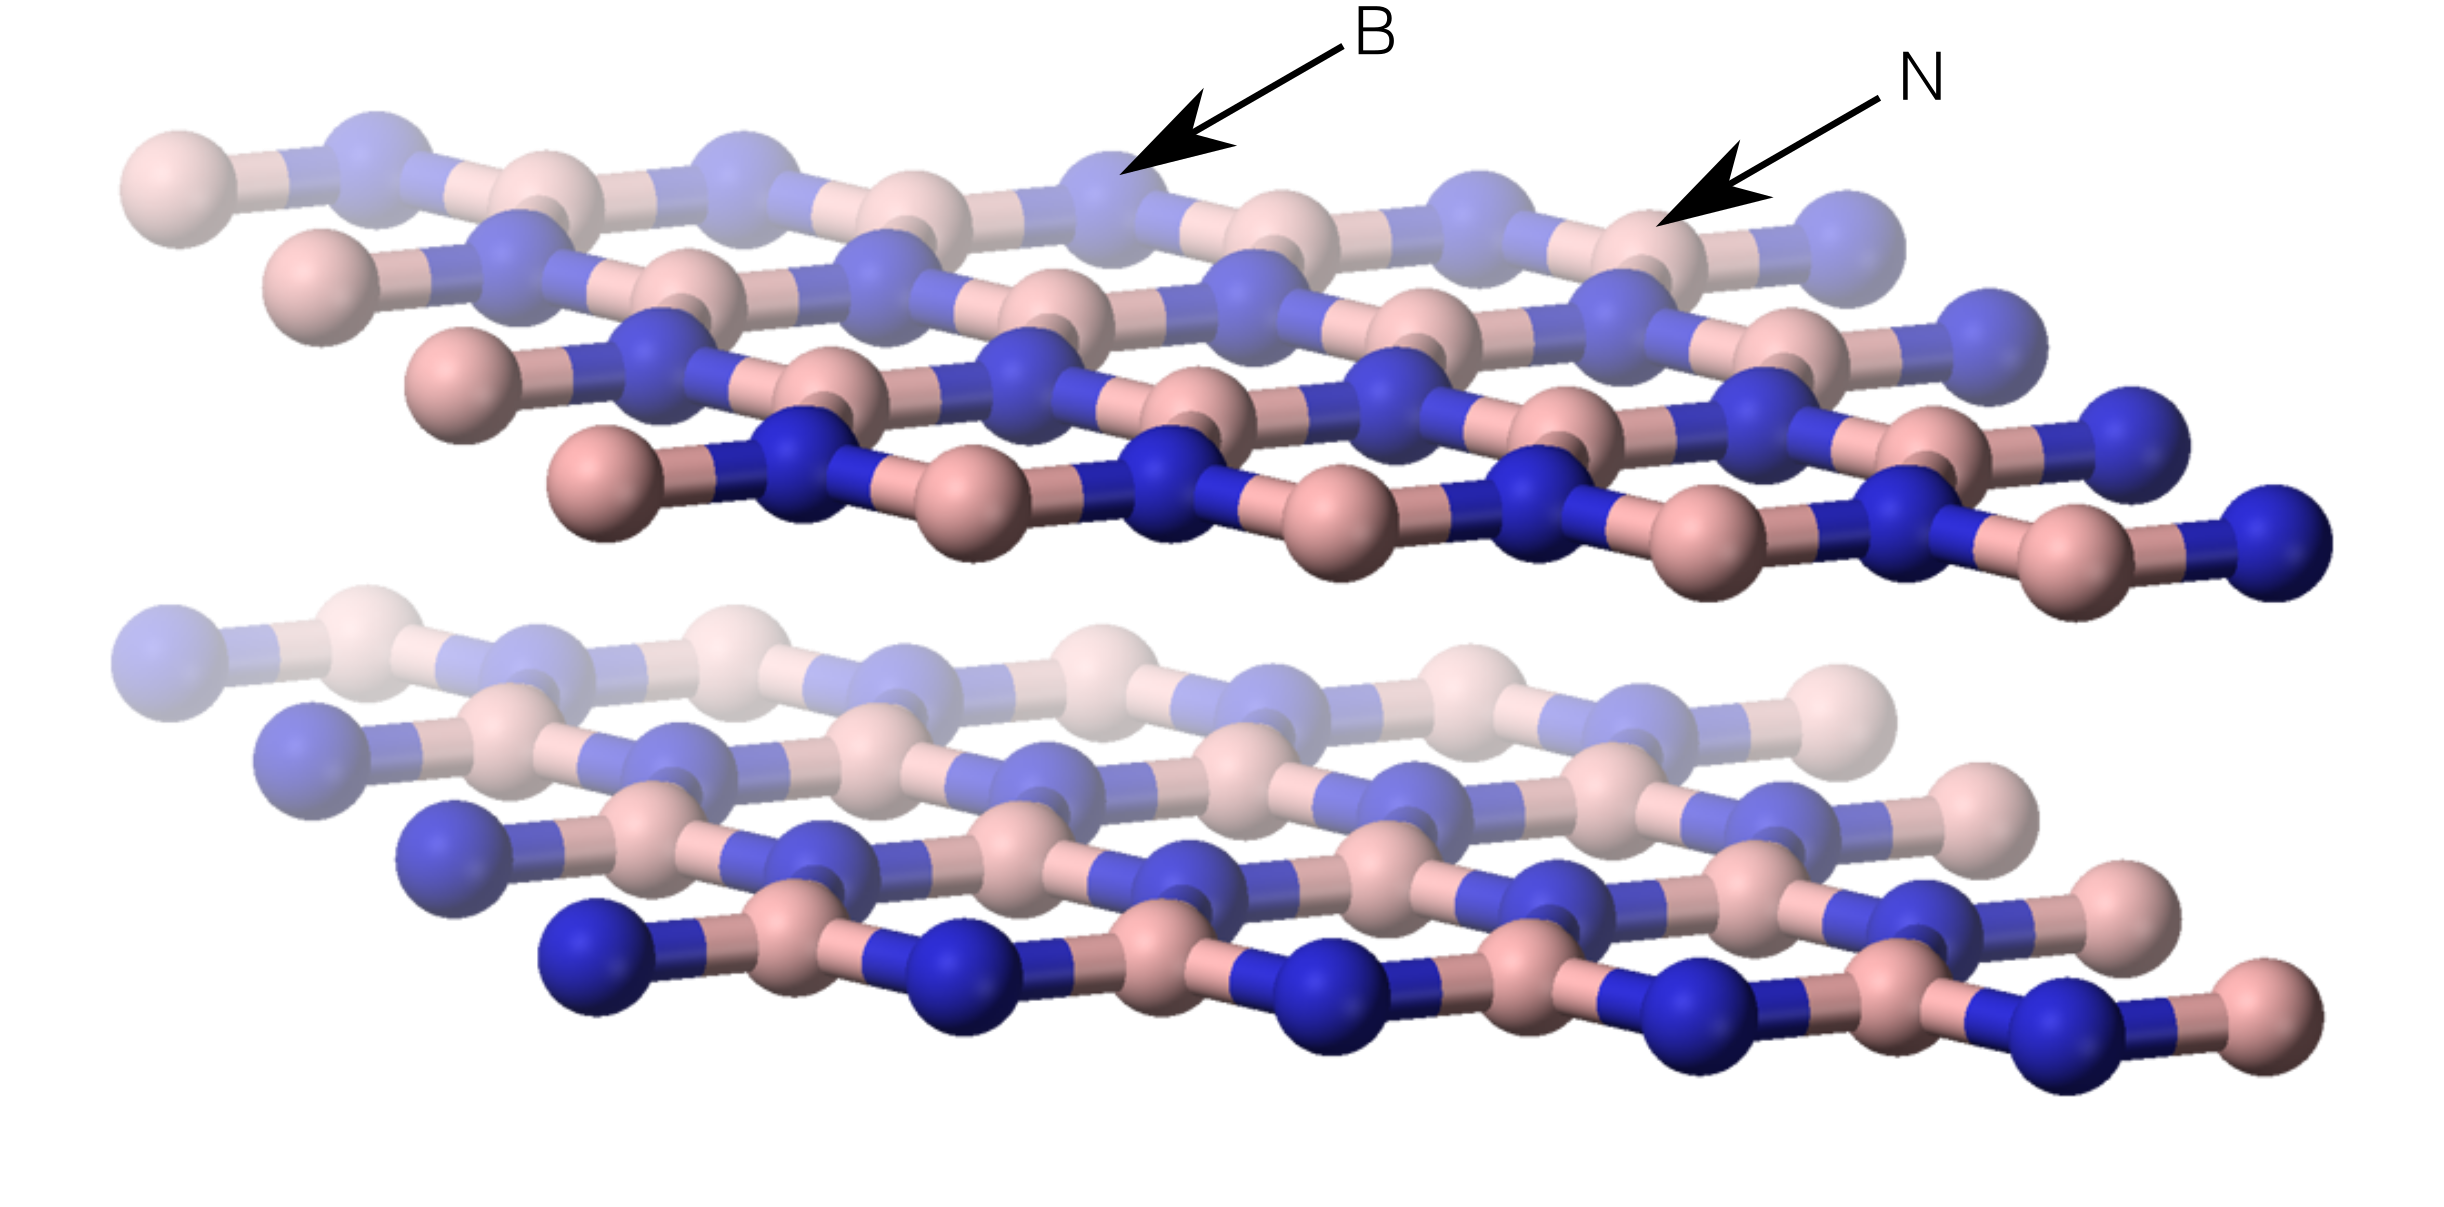
\includegraphics[width=0.9\textwidth]{BN.png}
\caption{Layered hexagonal crystal structures of BN. Image adapted from:\cite{Benjah2007}}  
\label{fig:BN}
\end{figure} 


\subsubsection{Transition Metal Dichalcogenides}

\begin{figure}[htbp!] 
\centering  
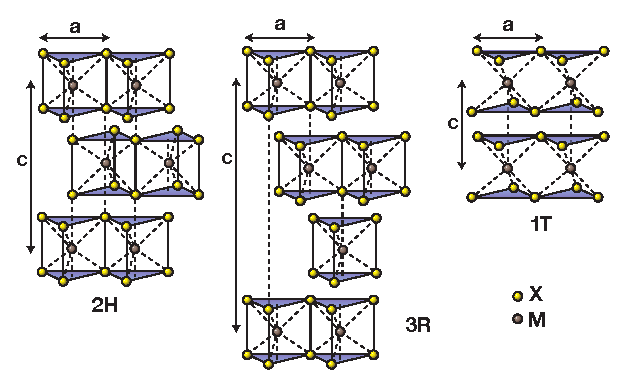
\includegraphics[width=0.9\textwidth]{tmds.eps}
\caption[Layered structures of TMDs]{Layered structures of TMDs. 2H: two layers per unit cell with hexagonal symmetry; 3R: three layers per unit cell with rhombohedral symmetry; 1T: one layer per unit cell with tetragonal symmetry. $a$ is the in-plane lattice constant with a range from 3.1 to 3.7 \AA~in TMDs. $c$ is the vertical lattice constant. The interlayer distance has a typical length of 6.5 \AA. Image source: \cite{Wang2012}}  
\label{fig:tmds}
\end{figure} 

Transition metal dichalcogenides (TMDs) have a generalized formula of MX$_2$, where M stands for the group 4-7 elements in the transition metal series in the periodic table, and X are the group VI elements. This is another type of layered materials, and the single layer of some of them have been experimentally realized.  These materials typical exist in three different structural phases as shown in \autoref{fig:tmds}, which at monolayer level can be either H or T phase. One of the most important differences in these two phases is the lack of inversion symmetry in H phase while T phase has it. Therefore, spin orbit coupling (SOC) is much important in H to induce spin-splitting than that in T phase, for instance 456 meV spin splitting in WSe$_2$\cite{Zhu2011giant} has been reported. Note that, inversion symmetry is recovered in the layered bulk form hence suppresses SOC. Another important consequence of reduce dimensionality is the indirect-to-direct band gap transition from layered TMDs to its 2D counterpart, see for example in \autoref{fig:tmds_bands}. 2D-TMDs have a broad range of potential applications. Electrocatalysis\cite{kim2013enhanced,huang2014synthesis} benefit from adequate active sites, electronic devices\cite{RadisavljevicB2011,sun2014fabrication} benefit from typical band gap of 1-2 eV, Li or Na batteries\cite{chang2011cysteine,chen2013situ} benefit from high surface-to-volume ratio and short diffusion path, photocatalysis benefit from high stability under extreme light intensity\cite{Li2013,Parzinger2015}, and biomedicine benefit from enhancement of the physiological stability and biocompatibility of polymers on 2D-TMDs\cite{Cheng2014,Yin2014}. 



\begin{figure}[htbp!] 
\centering  
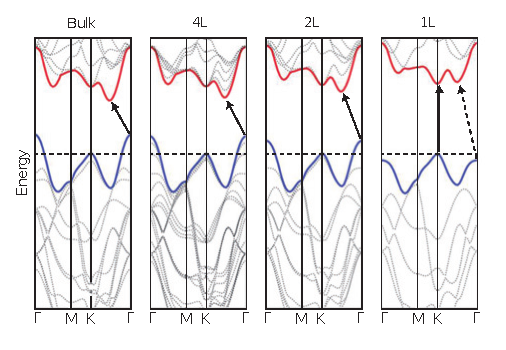
\includegraphics[width=0.9\textwidth]{tmds_bands.eps}
\caption{Band structure evolution of MoS$_2$ from bulk to single layer. Image source: \cite{Chhowalla2013}}  
\label{fig:tmds_bands}
\end{figure} 


\section{1D from 2D: nanotubes and nanoribbons}

The reduction of dimensionality of the materials did not stop at the 2D level. Further lowing it will result in 1D nanotubes or nanoribbons. 

\begin{figure}[htbp!] 
\centering  
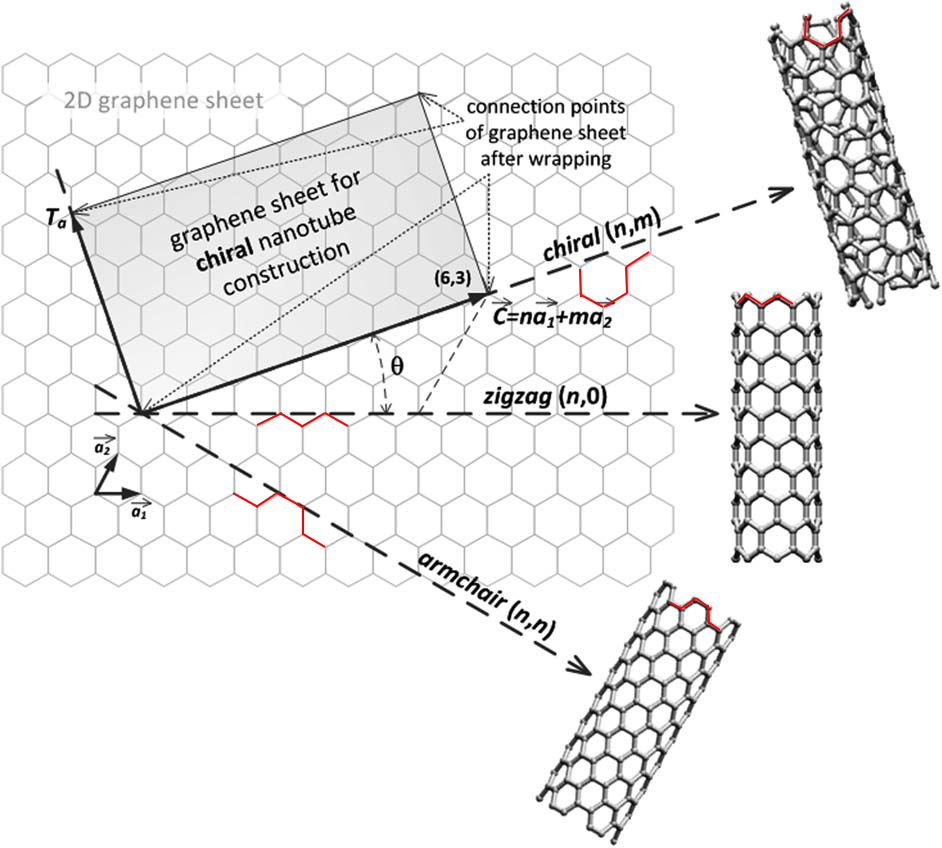
\includegraphics[width=0.8\textwidth]{chiral_vector.png}
\caption{Chiral vector and different type of nanotubes. Image adapted from \cite{Prasek2011}}  
\label{fig:chiral}
\end{figure} 

A nanoribbon is a strip of 2D sheet with nano-scale width and micro-scale length and it is still flat. Whereas nanotubes are the rolling up of nanoribbons to have a tube structure. Each nanotube, also each nanoribbon but with different definition, is associate with a chiral vector that uniquely define its structure parameters expect the length which is consider to be infinite in theory. In the \autoref{fig:chiral}, $a_1$ and $a_2$ are the unit lattice vectors in graphene.  Chiral vector, $\vec{C}$, is the superposition of these two unit vectors with indices pair ($n$,$m$). Zigzag edge always has a ($n$,0) form and ($n$,$n$) is always armchair edge. Everything else is called chiral type edge.  This finite-length chiral vector also define the radius of the tube. Nanoribbons, on the other hand, have these three types of edges as well. However, in this case, edges have infinite length. 

With confinements from other directions, physical properties of these system are expected to be different than that in their higher dimension counterparts. For example, graphene nanoribbons have a finite band gap as contrast to zero band gap in graphene\cite{Wang2008}. Moreover, control of this confinement will give tunable physical properties. For example, overall inverse band gap relation with the width of nanoribbon\cite{Han2007}. The zigzag edges in graphene nanoribbon form spin-polarized magnetic states give ferromagnetic ordering along the edge and anti-ferromagnetic ordering across edges\cite{Son2006}. For nanotubes, those have same edges belong to the same class of chirality and have same electronic structure. For instance, armchair carbon nanotubes are metallic, other types are semiconducting. But small radius tubes can be exceptional due to large curvature\cite{Bandaru2007}.  The strong mechanical strength and high thermal conductivity of graphene nanoribbon similar to those in graphene.

\section{Synthesis methods}

In this last section, I will briefly discuss some of the well-known synthesis methods for 2D materials. In \autoref{fig:syn}, a overview of graphene production methods is displayed in \autoref{fig:syn}. 

\begin{figure}[htbp!] 
\centering  
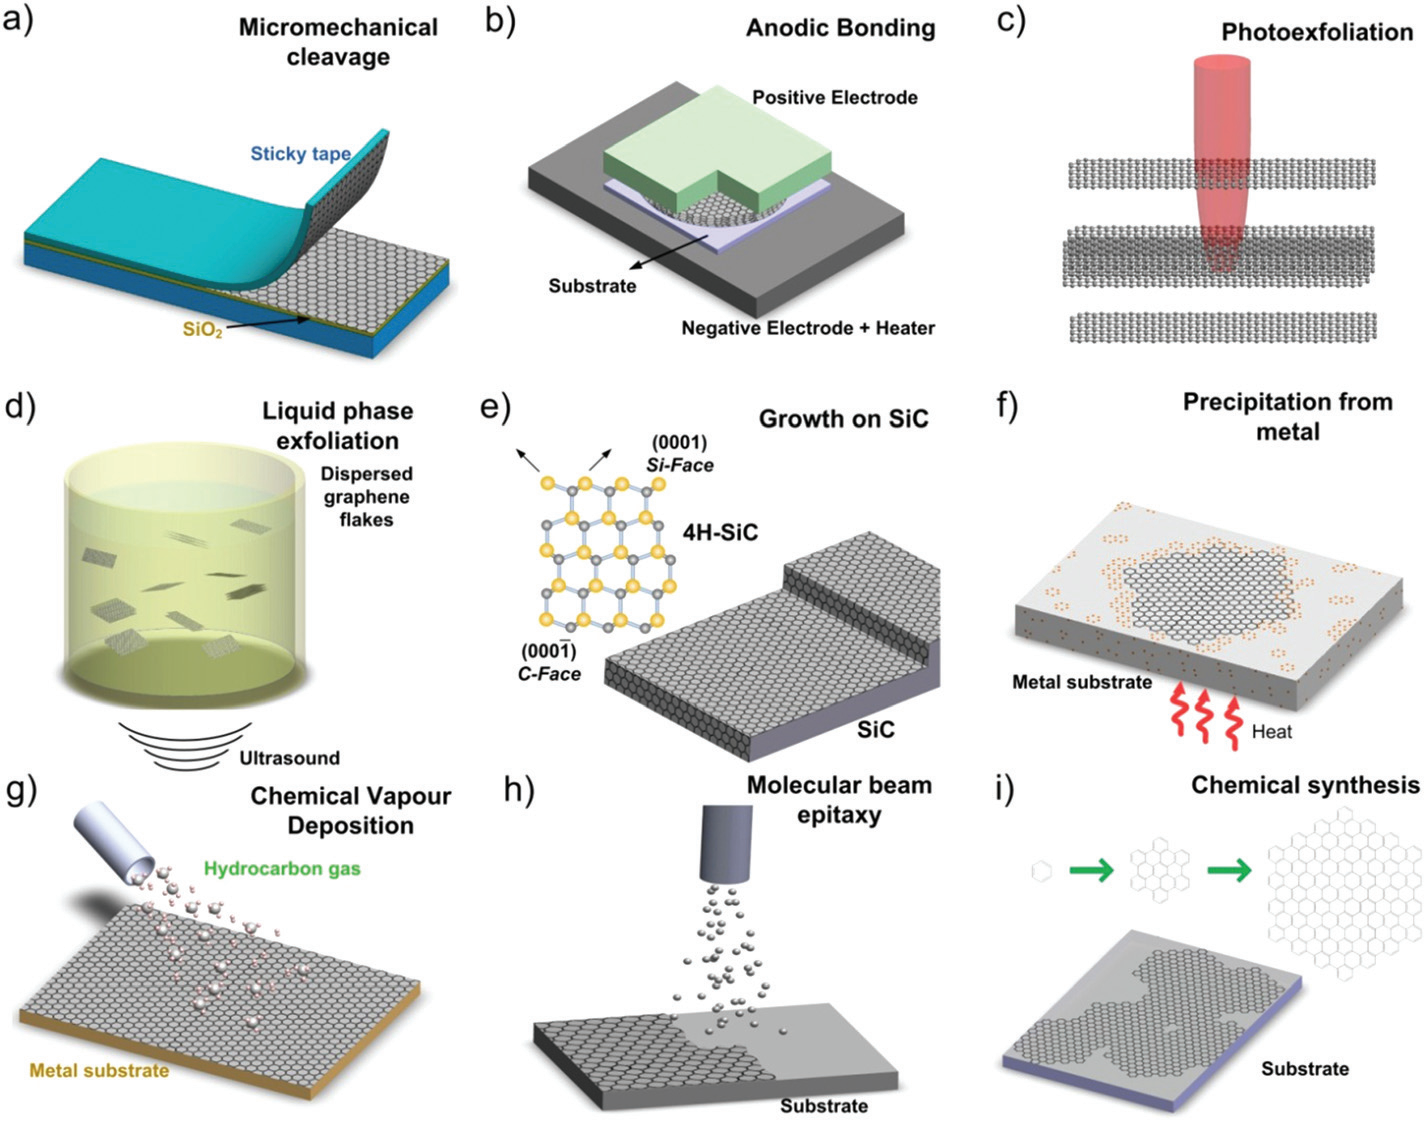
\includegraphics[width=\textwidth]{synthesis.png}
\caption{Graphene production setups. Image source \cite{Ferrari2015}}  
\label{fig:syn}
\end{figure} 
\subsubsection{Micromechanical cleavage}

Micromechanical cleavage is also known as mechanical exfoliation, which was the method used to first successful isolation of graphene in 2004 using a adhesive tape\cite{Novoselov26072005}. It involves separating layers in layered materials by mechanical, electrostatic, or electromagnetic forces. This method gives high quality product and suitable for laboratory-scale sample for fundamental studies. Large scale productions are impractical through this method.  Room temperature mobility was measured up to 20,000 cm$^2$V$^{-1}$s$^{-1}$\cite{Ni2010} on graphene prepared with this method.

\subsubsection{Liquid phase exfoliation}

Liquid phase exfoliation is the extraction of layers in a proper solvent using ultrasounds. The cavitation-induced bubbles collapse around the graphite will generate compressive stress wave. As a primary result, this will cause a reflective tensile wave whose strength is proportional with the number of such bubbles. Intensive tensile stress is enough to break graphite into graphite flakes. Additionally, as a secondary effect, shear effect can be develop from unbalance lateral stress, and separate two adjacent layers. Liquid phase exfoliation is a promising method to synthesis cheap and scalable samples. 

\subsubsection{Growth on SiC}

Growth of graphene on SiC involves Sic sample annealing at high temperature ( > 1400\si{\celsius}) in vacuum or under atmospheric pressure. The sublimation of silicon atoms leave behind carbon atoms on the surface which will rearrange to form graphitic layer\cite{Mishra2016}, see \autoref{fig:sic}. Apart from high reproducibility and production of homogeneous large-area sample of this method, it has an advantage that the graphene is available on semiconducting substrate for layer electronic device integration. 

\begin{figure}[htbp!] 
\centering  
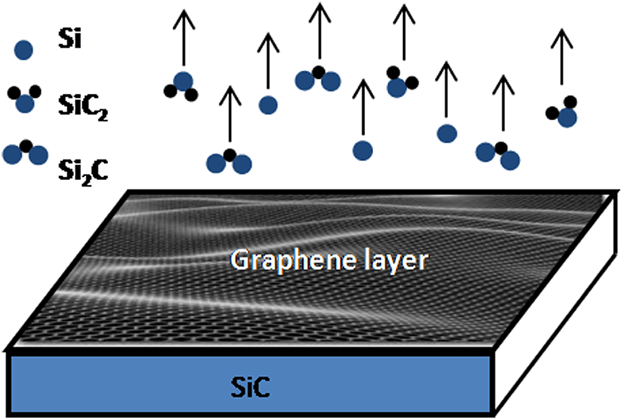
\includegraphics[width=0.6\textwidth]{gr-sic.png}
\caption{Growth of graphene on SiC wafer. Image source \cite{mishra2016graphene}}  
\label{fig:sic}
\end{figure} 

\subsubsection{Chemical vapor deposition}

Chemical vapor deposition (CVD) is a popular method to grow amorphous or crystalline thin film from solid, gaseous or liquid precursors. It is a direct deposition of vaporized desire material onto a particular substrate. Various of CVD methods exist depending on their operating pressure, types of vaporization and whether it is plasma-assisted etc.. Graphene grown on transition metals usually has a high quality. Carbon atoms from organic sources in the gas phase are deposited on metal (Ni, Ru, Ir etc.) and convert to graphene at high temperature. Then, for the characterization, graphene will be transferred to a proper substrate. Typical mobility of such type of sample is around 1000-25000 cm$^2$V$^{-1}$s$^{-1}$\cite{Petrone2012}. A 30-inch graphene film has been produced from roll-to-roll production through CVD methods by \citet{Bae2010}, see \autoref{fig:30gr}. The product measured to be a better electrode than commercially available indium tin oxides.

\begin{figure}[htbp!] 
\centering  
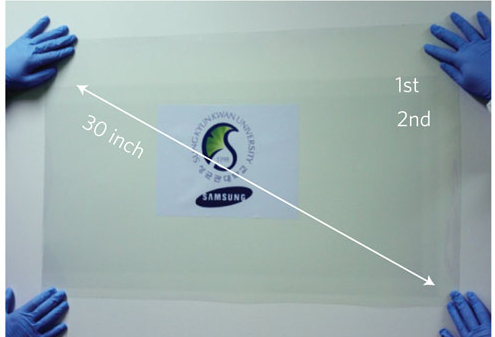
\includegraphics[width=0.7\textwidth]{30-inches-gr.jpg}
\caption{A ultra-large-area graphene film. Image source \cite{Bae2010}}  
\label{fig:30gr}
\end{figure} 

